\documentclass[conference]{IEEEtran}

% ---------- Packages ----------
\usepackage[T1]{fontenc}
\usepackage[utf8]{inputenc}
\usepackage{lmodern}
\usepackage{cite}
\usepackage{microtype}
\usepackage{graphicx}
\usepackage{booktabs}
\usepackage{array}
\usepackage{tabularx}
\usepackage{hyperref}
\usepackage{xcolor}
\usepackage{amsmath}
\usepackage{enumitem}
\usepackage{listings}
\usepackage{tikz}
\usepackage{pgfplots}
\usepackage{dblfloatfix}
\usepackage{placeins}
\usepackage{float}
\usetikzlibrary{positioning,arrows.meta,shapes.geometric,fit,calc}
\pgfplotsset{compat=1.18}

% ---------- Hyperref ----------
\hypersetup{
  colorlinks=false,
  hidelinks
}

% ---------- Listings ----------
\lstset{
  basicstyle=\ttfamily\small,
  breaklines=true,
  breakatwhitespace=false,
  frame=single,
  captionpos=b,
  float,
  floatplacement=tb,
  aboveskip=6pt,
  belowskip=6pt,
  linewidth=\columnwidth,
  xleftmargin=0.25em,
  framexleftmargin=0.25em,
  backgroundcolor=\color{black!3},
  columns=fullflexible
}

% Float spacing (tighter to avoid blank columns/pages)
\setlength{\textfloatsep}{8pt plus 2pt minus 2pt}
\setlength{\floatsep}{6pt plus 2pt minus 2pt}
\setlength{\intextsep}{6pt plus 2pt minus 2pt}

% ---------- Title ----------
\title{ScropIDS: A Multi-Tenant Cloud-Native Intrusion Detection Platform\\with Scheduler-Driven Aggregation and LLM-Assisted Threat Triage}
\author{\IEEEauthorblockN{Konda Nagendar}
\IEEEauthorblockA{Independent Researcher}}
\date{}

\begin{document}
\maketitle

\begin{abstract}
This paper presents ScropIDS, a production-oriented Intrusion Detection System (IDS) platform designed as a multi-tenant Software-as-a-Service (SaaS) application. The solution integrates cross-platform endpoint agents, secure event ingestion, scheduler-controlled aggregation, and large language model (LLM)-assisted alert analysis. Unlike traditional IDS workflows that expose analysts to high-volume raw logs, ScropIDS transforms telemetry into structured windows and JSON-based threat summaries, enabling faster triage and consistent decision support. The platform is implemented with Django, Celery, PostgreSQL, Redis, and a React TypeScript frontend, and is deployable through Docker Compose for local and cloud environments.
\end{abstract}

\begin{IEEEkeywords}
intrusion detection, multi-tenant SaaS, endpoint telemetry, alert triage, LLM security, scheduling, aggregation
\end{IEEEkeywords}

\section{Introduction}
Organizations rely on endpoint telemetry for early attack detection, yet practical IDS deployments face common barriers: heterogeneous data formats, noisy alerts, weak explainability, and poor usability. ScropIDS addresses these problems by combining:
\begin{itemize}[leftmargin=1.2em]
    \item cross-platform agent collection,
    \item strict event normalization,
    \item configurable scheduler and aggregation policies,
    \item LLM-assisted reasoning in machine-validated JSON,
    \item modern dashboard-driven operations.
\end{itemize}
The project goal is to provide a robust IDS platform that remains technically rigorous while being simple for analysts and administrators.

\section{Problem Statement and Motivation}
Security teams need early, reliable detection signals, but typical IDS deployments generate noisy outputs that are hard to interpret and difficult to operationalize. Multi-tenant SaaS environments further complicate deployment because data isolation, secure enrollment, and consistent agent configuration must be enforced across tenants. ScropIDS is motivated by three practical goals:
\begin{itemize}[leftmargin=1.2em]
    \item reduce analyst overhead by providing aggregated, structured summaries,
    \item maintain tenant isolation and secure onboarding in shared infrastructure,
    \item provide a usable dashboard experience for daily monitoring and response.
\end{itemize}

\section{Scope and Requirements}
\subsection{Functional Requirements}
\begin{itemize}[leftmargin=1.2em]
    \item Collect endpoint telemetry from Windows, Linux, and macOS.
    \item Support secure enrollment using one-time tokens or org access tokens.
    \item Ingest event batches and store normalized JSON records.
    \item Schedule aggregation and analysis at configurable intervals.
    \item Generate alerts with severity, confidence, and reasoning.
    \item Provide a dashboard for alerts, agents, and configuration.
\end{itemize}

\subsection{Non-Functional Requirements}
\begin{itemize}[leftmargin=1.2em]
    \item Secure data isolation per tenant and role.
    \item Stable operation under high-volume event ingestion.
    \item Maintainability with modular services and clear API boundaries.
    \item Portability via containerized deployment.
    \item Explainability of alert decisions and LLM output.
\end{itemize}

\section{Related Work}
Traditional IDS and SIEM pipelines emphasize high-volume log collection and rule evaluation, but they often lack consistent schema normalization and analyst-friendly explanations. Modern security products also integrate endpoint detection and response (EDR) features to provide richer context for investigations. ScropIDS aligns with these directions by emphasizing structured telemetry, rules-first triage, and explainable alert summaries. Industry frameworks such as MITRE ATT\&CK and Sigma rules inform detection coverage and vocabulary in many security systems, while NIST CSF provides governance guidance for security operations. ScropIDS builds on these foundations with a cloud-native, multi-tenant architecture to enable shared infrastructure without shared data exposure.

\section{Threat Model and Assumptions}
ScropIDS is designed to detect suspicious activity occurring on endpoints and within outbound network behavior. It assumes:
\begin{itemize}[leftmargin=1.2em]
    \item Agents can securely authenticate to the backend API.
    \item Endpoint OS audit sources are available and permitted by the administrator.
    \item Attackers may attempt process abuse, credential guessing, unauthorized remote access, or unusual outbound connections.
    \item The system is not intended to replace a full EDR suite, but to provide actionable IDS-level insights with explainable alerts.
\end{itemize}

\section{System Objectives}
\textbf{O1:} Support Windows/Linux/macOS endpoint telemetry. \\
\textbf{O2:} Ensure multi-tenant isolation and secure ingestion. \\
\textbf{O3:} Reduce alert fatigue via aggregation and rule-based triage. \\
\textbf{O4:} Integrate both API-hosted and local LLM inference providers. \\
\textbf{O5:} Deliver operational visibility through a responsive web console.

\section{Project Contributions}
This work contributes:
\begin{itemize}[leftmargin=1.2em]
    \item a cross-platform agent-to-cloud pipeline with strict JSON normalization,
    \item a scheduler-driven aggregation and triage workflow that reduces alert noise,
    \item a dual-mode LLM integration layer with reliable schema validation,
    \item a production-ready web console tailored to IDS workflows,
    \item a reproducible deployment model for local and cloud environments.
\end{itemize}

\section{Repository and Implementation Overview}
The project is organized as a monorepo with separate backend, frontend, and agent modules. This layout supports independent development while keeping the deployment model consistent.
\begin{lstlisting}[caption={Repository layout (abridged)}]
backend/     # Django API, scheduler, pipeline
frontend/    # React + Vite dashboard
agents/go/   # Go agent starter
docs/        # Architecture and API docs
docker-compose.yml
Report.tex
\end{lstlisting}

\section{Architecture Overview}
\subsection{High-Level Component Design}
\begin{figure}[!t]
\centering
\resizebox{\columnwidth}{!}{%
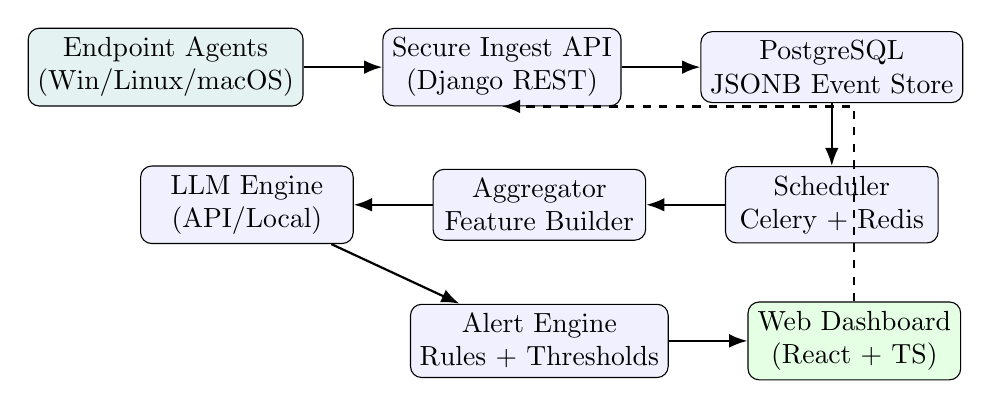
\begin{tikzpicture}[
  node distance=8mm and 10mm,
  box/.style={draw, rounded corners, minimum width=27mm, minimum height=9mm, align=center, fill=blue!6},
  arr/.style={-Latex, thick}
]
\node[box, fill=teal!10] (agent) {Endpoint Agents\\(Win/Linux/macOS)};
\node[box, right=of agent] (ingest) {Secure Ingest API\\(Django REST)};
\node[box, right=of ingest] (db) {PostgreSQL\\JSONB Event Store};
\node[box, below=of db] (sched) {Scheduler\\Celery + Redis};
\node[box, left=of sched] (agg) {Aggregator\\Feature Builder};
\node[box, left=of agg] (llm) {LLM Engine\\(API/Local)};
\node[box, below=of agg] (alert) {Alert Engine\\Rules + Thresholds};
\node[box, right=of alert, fill=green!10] (ui) {Web Dashboard\\(React + TS)};

\draw[arr] (agent) -- (ingest);
\draw[arr] (ingest) -- (db);
\draw[arr] (db) -- (sched);
\draw[arr] (sched) -- (agg);
\draw[arr] (agg) -- (llm);
\draw[arr] (llm) -- (alert);
\draw[arr] (alert) -- (ui);
\draw[arr, dashed] (ui.north) |- (ingest.south);
\end{tikzpicture}}
\caption{ScropIDS end-to-end architecture.}
\label{fig:architecture}
\end{figure}

\subsection{Processing Pipeline}
\begin{enumerate}[leftmargin=1.2em]
    \item Agent collects events (process, auth, network, file, system).
    \item Events are normalized and sent via HTTPS.
    \item Backend validates and stores event JSON.
    \item Scheduler triggers window aggregation.
    \item Aggregates are scored by rules and optionally sent to LLM.
    \item Alert engine creates incidents based on threshold policy.
    \item Dashboard renders real-time analyst views.
\end{enumerate}

\subsection{Data Lifecycle and Storage Flow}
\begin{figure}[!t]
\centering
\resizebox{\columnwidth}{!}{%
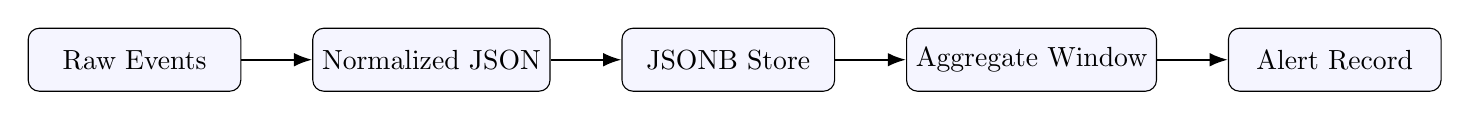
\begin{tikzpicture}[
  node distance=7mm and 9mm,
  box/.style={draw, rounded corners, minimum width=27mm, minimum height=8mm, align=center, fill=blue!4},
  arr/.style={-Latex, thick}
]
\node[box] (raw) {Raw Events};
\node[box, right=of raw] (norm) {Normalized JSON};
\node[box, right=of norm] (store) {JSONB Store};
\node[box, right=of store] (win) {Aggregate Window};
\node[box, right=of win] (alert) {Alert Record};

\draw[arr] (raw) -- (norm);
\draw[arr] (norm) -- (store);
\draw[arr] (store) -- (win);
\draw[arr] (win) -- (alert);
\end{tikzpicture}}
\caption{Event lifecycle from ingestion to alert creation.}
\label{fig:lifecycle}
\end{figure}

\subsection{Enrollment and Authentication Flow}
\begin{figure}[!t]
\centering
\resizebox{\columnwidth}{!}{%
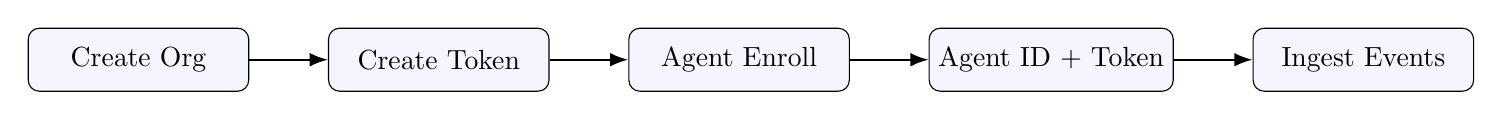
\begin{tikzpicture}[
  node distance=6mm and 10mm,
  box/.style={draw, rounded corners, minimum width=28mm, minimum height=8mm, align=center, fill=blue!4},
  arr/.style={-Latex, thick}
]
\node[box] (org) {Create Org};
\node[box, right=of org] (token) {Create Token};
\node[box, right=of token] (enroll) {Agent Enroll};
\node[box, right=of enroll] (creds) {Agent ID + Token};
\node[box, right=of creds] (ingest) {Ingest Events};

\draw[arr] (org) -- (token);
\draw[arr] (token) -- (enroll);
\draw[arr] (enroll) -- (creds);
\draw[arr] (creds) -- (ingest);
\end{tikzpicture}}
\caption{Enrollment flow for tenant onboarding and agent authentication.}
\label{fig:enrollment}
\end{figure}

\subsection{Multi-Tenant Isolation}
Tenant isolation is enforced through organization ownership on every core record (agents, events, aggregates, alerts). The API resolves a tenant from the authenticated user and optional \texttt{X-Organization-Slug} header, ensuring that dashboard queries only access permitted data.

\section{Data Model and JSON Normalization}
Core entities include \texttt{Organization}, \texttt{Agent}, \texttt{Event}, \texttt{AggregatedWindow}, \texttt{Alert}, \texttt{LLMProviderConfig}, and \texttt{SchedulerConfig}.  
A representative normalized event format is shown below.

\begin{table}[!t]
\centering
\begin{tabular}{ll}
\toprule
\textbf{Entity} & \textbf{Purpose} \\
\midrule
Organization & Tenant boundary and access scope \\
Agent & Endpoint identity and status \\
Event & Normalized telemetry record \\
AggregatedWindow & Time-bucketed feature summary \\
Alert & Triage artifact with severity and status \\
LLMProviderConfig & Model settings and API details \\
SchedulerConfig & Aggregation and analysis policy \\
\bottomrule
\end{tabular}
\caption{Core data model entities.}
\label{tab:entities}
\end{table}

\begin{lstlisting}[language=json,caption={Normalized endpoint event schema}]
{
  "agent_id": "mac-001",
  "timestamp": "2026-03-14T10:40:22Z",
  "event_type": "process_creation",
  "severity": "high",
  "source": "process_monitor",
  "data": {
    "process_name": "python3",
    "command_line": "python3 -c \"import base64;...\"",
    "parent_process": "zsh",
    "user": "nagender"
  }
}
\end{lstlisting}

\subsection{Event Schema Fields}
\begin{table}[!t]
\centering
\begin{tabular}{>{\raggedright\arraybackslash}p{0.32\columnwidth} >{\raggedright\arraybackslash}p{0.58\columnwidth}}
\toprule
\textbf{Field} & \textbf{Description} \\
\midrule
timestamp & Event time (ISO 8601) \\
event\_type & Category of telemetry (process, auth, network) \\
severity & Normalized severity label \\
source & Collector origin \\
data & Event-specific payload \\
\bottomrule
\end{tabular}
\caption{Core fields in the normalized event schema.}
\label{tab:event-fields}
\end{table}

\subsection{Aggregate Summary Example}
Aggregated windows store concise features such as counts and top offenders. These summaries are optimized for both rule checks and LLM prompts.
\begin{lstlisting}[language=json,caption={Aggregated window example}]
{
  "agent_id": "mac-001",
  "window_start": "2026-03-14T10:40:00Z",
  "window_end": "2026-03-14T10:45:00Z",
  "summary": {
    "failed_logins": 12,
    "new_processes": 45,
    "suspicious_commands": 3,
    "external_connections": 8
  }
}
\end{lstlisting}
\FloatBarrier

\section{Agent Architecture}
ScropIDS uses a Go-based agent starter that supports interactive setup and scheduled telemetry collection. The agent stores configuration locally, periodically refreshes runtime settings from the server, and batches events for efficient ingestion.

\subsection{Agent Modules}
\begin{figure}[!t]
\centering
\resizebox{\columnwidth}{!}{%
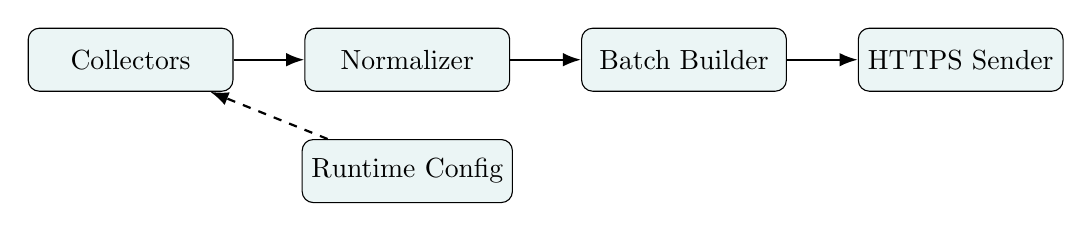
\begin{tikzpicture}[
  node distance=6mm and 9mm,
  box/.style={draw, rounded corners, minimum width=26mm, minimum height=8mm, align=center, fill=teal!8},
  arr/.style={-Latex, thick}
]
\node[box] (collect) {Collectors};
\node[box, right=of collect] (norm) {Normalizer};
\node[box, right=of norm] (batch) {Batch Builder};
\node[box, right=of batch] (send) {HTTPS Sender};
\node[box, below=of norm] (config) {Runtime Config};

\draw[arr] (collect) -- (norm);
\draw[arr] (norm) -- (batch);
\draw[arr] (batch) -- (send);
\draw[arr, dashed] (config) -- (collect);
\end{tikzpicture}}
\caption{Agent module flow.}
\label{fig:agent-modules}
\end{figure}

\subsection{Collectors}
\begin{table}[!t]
\centering
\begin{tabular}{>{\raggedright\arraybackslash}p{0.33\columnwidth} >{\raggedright\arraybackslash}p{0.58\columnwidth}}
\toprule
\textbf{Collector} & \textbf{Signal Type} \\
\midrule
Process snapshot & New or suspicious processes \\
Security signals & Authentication or access anomalies \\
Network snapshot & Outbound connections and ports \\
System snapshot & Host metadata and uptime \\
File watch & Burst file changes (optional) \\
\bottomrule
\end{tabular}
\caption{Agent collectors implemented in the Go starter.}
\label{tab:collectors}
\end{table}

\subsection{Agent Configuration and Scheduling}
Agents maintain a local configuration file and can run in a guided setup mode. They fetch the runtime profile from \texttt{/api/v1/ingest/config/}, which includes collector toggles and event intervals. This allows centralized policy updates without redeploying binaries.
\FloatBarrier

\section{Backend Architecture}
The backend is a Django REST application with multi-tenant data models, API endpoints, and a scheduler-driven pipeline.

\subsection{Core Models}
The core data model includes \texttt{Organization}, \texttt{OrganizationMembership}, \texttt{AgentEnrollmentToken}, \texttt{Agent}, \texttt{Event}, \texttt{SchedulerConfig}, \texttt{LLMProviderConfig}, \texttt{AggregatedWindow}, and \texttt{Alert}. Each record is linked to a tenant organization to enforce isolation.

\subsection{Multi-Tenant Access Control}
Tenant selection occurs through membership lookup and the optional \texttt{X-Organization-Slug} header. Viewsets restrict queries to organizations associated with the authenticated user, and agent ingestion uses opaque agent credentials to map events to a tenant.

\subsection{Secure Secret Storage}
Provider API keys and organization access tokens are stored encrypted at rest. Encryption is handled by a backend service using Fernet, minimizing exposure of plaintext credentials.

\subsection{Alerting and Notifications}
Alerts are generated when LLM outputs or rules exceed tenant thresholds. Optional outbound channels include email and webhook-style notifiers. These are configured via environment variables.
\FloatBarrier

\section{API Contract Summary}
Table \ref{tab:api} summarizes the primary API endpoints. All dashboard endpoints are tenant-scoped and respect the optional \texttt{X-Organization-Slug} header.
\begin{figure}[!t]
\centering
\resizebox{\columnwidth}{!}{%
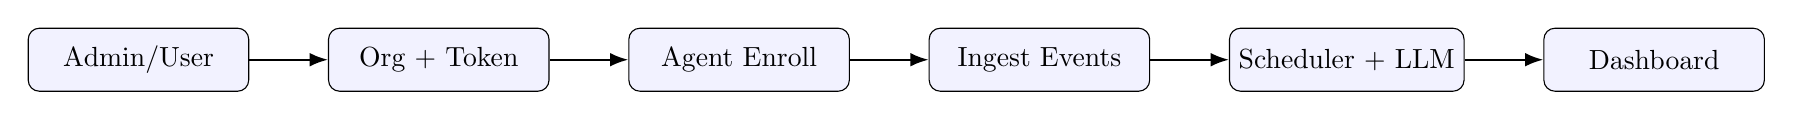
\begin{tikzpicture}[
  node distance=7mm and 10mm,
  box/.style={draw, rounded corners, minimum width=28mm, minimum height=8mm, align=center, fill=blue!5},
  arr/.style={-Latex, thick}
]
\node[box] (admin) {Admin/User};
\node[box, right=of admin] (org) {Org + Token};
\node[box, right=of org] (agent) {Agent Enroll};
\node[box, right=of agent] (ingest) {Ingest Events};
\node[box, right=of ingest] (sched) {Scheduler + LLM};
\node[box, right=of sched] (dash) {Dashboard};

\draw[arr] (admin) -- (org);
\draw[arr] (org) -- (agent);
\draw[arr] (agent) -- (ingest);
\draw[arr] (ingest) -- (sched);
\draw[arr] (sched) -- (dash);
\end{tikzpicture}}
\caption{High-level API flow from tenant onboarding to alert visibility.}
\label{fig:api-flow}
\end{figure}

\begin{table}[!t]
\centering
\caption{Key API endpoints in ScropIDS (tenant and agent flows)}
\label{tab:api}
\small
\begin{tabularx}{\columnwidth}{l l X}
\toprule
\textbf{Method} & \textbf{Endpoint} & \textbf{Purpose} \\
\midrule
POST & \texttt{/api/v1/organizations/} & Create tenant organization \\
GET & \texttt{/api/v1/organizations/} & List organizations for user \\
GET & \texttt{/api/v1/organization-memberships/} & List user memberships \\
POST & \texttt{/api/v1/agent-enrollment-tokens/} & Create one-time enrollment token \\
GET & \texttt{/api/v1/agent-enrollment-tokens/} & List enrollment tokens \\
POST & \texttt{/api/v1/agents/enroll/} & Enroll agent with token \\
POST & \texttt{/api/v1/agents/quick-enroll/} & Enroll agent with org access token \\
POST & \texttt{/api/v1/agents/bootstrap/} & Admin bootstrap new agent \\
GET & \texttt{/api/v1/agents/access-token/} & Retrieve org access token \\
POST & \texttt{/api/v1/agents/access-token/} & Rotate org access token \\
GET & \texttt{/api/v1/agents/} & List agents for tenant \\
GET & \texttt{/api/v1/agents/\textless uuid\textgreater/timeline/} & Agent event timeline \\
POST & \texttt{/api/v1/ingest/events/} & Ingest event batch \\
POST & \texttt{/api/v1/ingest/heartbeat/} & Agent heartbeat \\
GET & \texttt{/api/v1/ingest/config/} & Agent runtime profile \\
GET & \texttt{/api/v1/agent-downloads/} & Agent package manifest \\
GET & \texttt{/api/v1/agent-downloads/\textless file\textgreater/} & Download agent package \\
\bottomrule
\end{tabularx}
\end{table}

\begin{table}[!t]
\centering
\caption{Key API endpoints in ScropIDS (dashboard and configuration)}
\label{tab:api-dashboard}
\small
\begin{tabularx}{\columnwidth}{l l X}
\toprule
\textbf{Method} & \textbf{Endpoint} & \textbf{Purpose} \\
\midrule
GET & \texttt{/api/v1/dashboard/overview/} & Dashboard metrics and charts \\
GET & \texttt{/api/v1/scheduler-configs/} & List scheduler configs \\
PATCH & \texttt{/api/v1/scheduler-configs/\textless id\textgreater/} & Update scheduler config \\
GET & \texttt{/api/v1/llm-providers/} & List LLM providers \\
POST & \texttt{/api/v1/llm-providers/} & Create LLM provider \\
PATCH & \texttt{/api/v1/llm-providers/\textless id\textgreater/} & Update LLM provider \\
GET & \texttt{/api/v1/alerts/} & List alerts \\
PATCH & \texttt{/api/v1/alerts/\textless id\textgreater/} & Update alert status \\
\bottomrule
\end{tabularx}
\end{table}
\FloatBarrier

\section{Implementation Details}
\subsection{Aggregation Window Design}
Events are grouped into time windows to create structured summaries for LLM analysis and rule evaluation. The aggregation step counts signals such as failed logins, suspicious commands, and external connections. This reduces volume and improves interpretability.

\subsection{Threat Level Mapping}
Threat levels are normalized into four categories: low, medium, high, and critical. The alert threshold comparison is applied after rule escalation to ensure deterministic alert creation even when LLM outputs are conservative.

\subsection{Alert Lifecycle}
\begin{figure}[!t]
\centering
\resizebox{\columnwidth}{!}{%
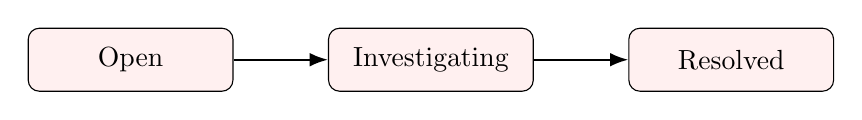
\begin{tikzpicture}[
  node distance=8mm and 12mm,
  box/.style={draw, rounded corners, minimum width=26mm, minimum height=8mm, align=center, fill=red!6},
  arr/.style={-Latex, thick}
]
\node[box] (open) {Open};
\node[box, right=of open] (investigate) {Investigating};
\node[box, right=of investigate] (resolved) {Resolved};

\draw[arr] (open) -- (investigate);
\draw[arr] (investigate) -- (resolved);
\end{tikzpicture}
}
\caption{Alert lifecycle states.}
\label{fig:alert-states}
\end{figure}

\subsection{Agent Packaging and Distribution}
Cross-platform agent artifacts are built from the Go codebase and stored in a backend download directory. The API exposes a manifest and file download endpoints, enabling users to obtain packages directly from the dashboard.

\subsection{Dashboard Data Flow}
The frontend periodically pulls \texttt{/api/v1/dashboard/overview/} to refresh KPIs and charts. Alert and agent views use list endpoints with tenant scoping, while configuration pages update scheduler and LLM provider settings via PATCH.

\section{Scheduler and Detection Logic}
\subsection{Server Scheduler}
Server-side policies define:
\begin{itemize}[leftmargin=1.2em]
    \item aggregation interval (e.g., 60--300 seconds),
    \item LLM mode (batch/real-time),
    \item minimum severity for analysis,
    \item alert threshold for incident creation.
\end{itemize}

\subsection{Agent Scheduler Profile}
Agent runtime profile can include:
\begin{itemize}[leftmargin=1.2em]
    \item sync interval,
    \item event batch interval,
    \item enabled collectors,
    \item elevated-permission mode.
\end{itemize}
This supports centralized control while allowing endpoint-level tuning.

\subsection{Rules and Heuristics}
In addition to LLM analysis, ScropIDS applies lightweight rules to flag high-risk patterns quickly.
\begin{table}[!t]
\centering
\begin{tabular}{>{\raggedright\arraybackslash}p{0.28\columnwidth} >{\raggedright\arraybackslash}p{0.50\columnwidth} >{\raggedright\arraybackslash}p{0.12\columnwidth}}
\toprule
\textbf{Rule} & \textbf{Signal} & \textbf{Severity} \\
\midrule
Credential Burst & Repeated auth failures & High \\
Suspicious CLI & Encoded or obfuscated commands & High \\
New External C2 & New outbound IP + uncommon port & Critical \\
Mass File Change & High write volume in short window & Medium \\
\bottomrule
\end{tabular}
\caption{Example detection rules used for fast triage.}
\label{tab:rules}
\end{table}

\subsection{Scheduler Tick Algorithm}
The scheduler runs as a Celery beat task and checks each tenant configuration before processing. The simplified logic below reflects the pipeline behavior.
\begin{lstlisting}[caption={Scheduler tick pseudocode}]
for each scheduler_config where scheduler_enabled:
    if interval not reached: continue
    aggregates = aggregate_events(organization, window_start, window_end)
    for each aggregate:
        llm_output = analyze_aggregate(aggregate.summary_json)
        llm_output = apply_rule_escalation(llm_output, aggregate.summary_json)
        save aggregate.llm_output
        if llm_output.threat_level >= alert_threshold:
            create alert
\end{lstlisting}

\subsection{Runtime Timeline}
\begin{figure}[!t]
\centering
\resizebox{\columnwidth}{!}{%
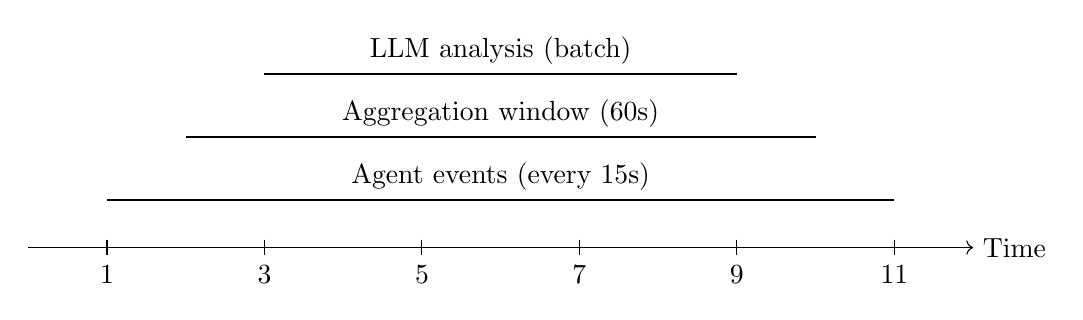
\begin{tikzpicture}[x=1cm,y=1cm]
  \draw[->] (0,0) -- (12,0) node[right] {Time};
  \foreach \x in {1,3,5,7,9,11} { \draw (\x,0.1) -- (\x,-0.1) node[below] {\x}; }
  \draw[thick] (1,0.6) -- (11,0.6);
  \node at (6,0.9) {Agent events (every 15s)};
  \draw[thick] (2,1.4) -- (10,1.4);
  \node at (6,1.7) {Aggregation window (60s)};
  \draw[thick] (3,2.2) -- (9,2.2);
  \node at (6,2.5) {LLM analysis (batch)};
\end{tikzpicture}}
\caption{Illustrative runtime scheduling cadence.}
\label{fig:timeline}
\end{figure}
\FloatBarrier

\section{LLM-Assisted Threat Analysis}
LLM integration supports OpenAI-compatible APIs and local runtimes. ScropIDS enforces JSON-only outputs for deterministic parsing.

\begin{lstlisting}[language=json,caption={Expected LLM response schema}]
{
  "threat_level": "low|medium|high|critical",
  "confidence": 0,
  "reasoning": "short explanation",
  "recommended_action": "clear mitigation step"
}
\end{lstlisting}

\textbf{Reliability controls:}
\begin{itemize}[leftmargin=1.2em]
    \item strict response parsing and schema validation,
    \item fallback classification when LLM fails or times out,
    \item audit logging of prompt-response lifecycle.
\end{itemize}

\subsection{Prompt Contract}
To reduce hallucinations and enforce parseable output, the platform uses an explicit schema contract and rejects non-JSON responses. This ensures deterministic handling in the alert engine and preserves auditability for later review.

\subsection{Provider Modes}
\begin{table}[!t]
\centering
\begin{tabular}{>{\raggedright\arraybackslash}p{0.33\columnwidth} >{\raggedright\arraybackslash}p{0.28\columnwidth} >{\raggedright\arraybackslash}p{0.30\columnwidth}}
\toprule
\textbf{Mode} & \textbf{Endpoint Type} & \textbf{Typical Use} \\
\midrule
OpenAI-compatible API & HTTPS JSON API & Cloud inference and hosted models \\
Ollama local & Local HTTP service & Offline or on-prem inference \\
\bottomrule
\end{tabular}
\caption{Supported LLM provider modes.}
\label{tab:llm-modes}
\end{table}

\subsection{Failure Handling}
If an LLM provider is unreachable or returns invalid JSON, the pipeline stores a fallback output and continues the scheduler run. This prevents complete pipeline failure while preserving visibility into the cause.
\FloatBarrier

\section{Security Controls}
\begin{itemize}[leftmargin=1.2em]
    \item tenant-scoped API access using organization context,
    \item session auth for dashboard users,
    \item encrypted secret storage for provider keys,
    \item transport security through HTTPS-ready deployment,
    \item role-aware administrative controls.
\end{itemize}
Data retention is handled at the database layer; organizations can define their own retention and backup strategies based on deployment policy.
\subsection{Authentication Modes}
\begin{itemize}[leftmargin=1.2em]
    \item Dashboard session authentication for human users.
    \item Agent token authentication for event ingestion.
    \item One-time enrollment tokens for controlled onboarding.
    \item Organization access tokens for rapid bulk enrollment.
\end{itemize}

\section{System Requirements and Constraints}
\begin{table}[!t]
\centering
\begin{tabular}{>{\raggedright\arraybackslash}p{0.34\columnwidth} >{\raggedright\arraybackslash}p{0.56\columnwidth}}
\toprule
\textbf{Component} & \textbf{Minimum Requirement} \\
\midrule
Backend & 2 vCPU, 4 GB RAM \\
Database & PostgreSQL 13+ with JSONB \\
Queue & Redis 6+ \\
Agent & OS audit access, TLS outbound \\
Frontend & Modern browser (Chromium/Firefox/Safari) \\
\bottomrule
\end{tabular}
\caption{Baseline requirements for local or small-scale deployment.}
\label{tab:reqs}
\end{table}

\section{User Interface Design}
The dashboard uses a dark IDS theme with high signal-to-noise visualization:
\begin{itemize}[leftmargin=1.2em]
    \item KPI cards (agents, events, active alerts, queue depth),
    \item severity distribution and confidence heatmaps,
    \item searchable alert/event feeds,
    \item scheduler + LLM configuration panels.
\end{itemize}

\subsection{Frontend Stack}
The UI is implemented with React, Vite, and TypeScript, styled with TailwindCSS and component patterns inspired by shadcn/ui. Charts use Recharts, and navigation is managed by React Router.

\subsection{Information Architecture}
\begin{figure}[!t]
\centering
\resizebox{\columnwidth}{!}{%
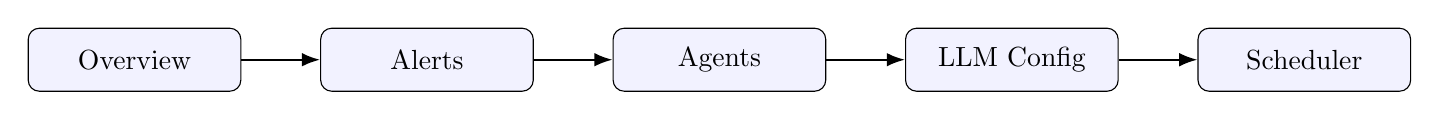
\begin{tikzpicture}[
  node distance=6mm and 10mm,
  box/.style={draw, rounded corners, minimum width=27mm, minimum height=8mm, align=center, fill=blue!5},
  arr/.style={-Latex, thick}
]
\node[box] (overview) {Overview};
\node[box, right=of overview] (alerts) {Alerts};
\node[box, right=of alerts] (agents) {Agents};
\node[box, right=of agents] (llm) {LLM Config};
\node[box, right=of llm] (sched) {Scheduler};

\draw[arr] (overview) -- (alerts);
\draw[arr] (alerts) -- (agents);
\draw[arr] (agents) -- (llm);
\draw[arr] (llm) -- (sched);
\end{tikzpicture}}
\caption{Primary dashboard navigation structure.}
\label{fig:ui-nav}
\end{figure}

\section{Operational Workflow Walkthrough}
This section summarizes the end-to-end flow that a tenant follows in a typical deployment:
\begin{enumerate}[leftmargin=1.2em]
    \item Create an organization (tenant) in the dashboard or via API.
    \item Generate a one-time enrollment token or org access token.
    \item Enroll the agent and obtain agent credentials.
    \item Send event batches and heartbeat signals.
    \item Scheduler aggregates events and triggers LLM analysis.
    \item Alerts are created and displayed in the dashboard.
\end{enumerate}

\section{Use Case Scenarios}
\subsection{Credential Abuse Detection}
Repeated authentication failures within a short window are aggregated into a high-severity signal. The system escalates this using rules and optionally corroborates it with LLM reasoning to recommend account lockout or MFA review.

\subsection{Suspicious Process Execution}
Encoded command-line execution or abnormal parent-child process relationships are flagged as high-risk. The resulting alert includes a recommendation to inspect process lineage and command arguments.

\subsection{Outbound Beaconing}
Unusual outbound connections to new destinations, especially on uncommon ports, are grouped and prioritized. The alert view highlights source host, destination IP, and potential containment steps.

\section{Configuration and Administration}
\subsection{Tenant Management}
Administrators can create organizations, manage memberships, and issue enrollment tokens. Each tenant receives a scheduler configuration profile that can be updated without restarting services.

\subsection{LLM Provider Configuration}
The LLM configuration page allows administrators to add providers, set model names, base URLs, and activation flags. Providers are tenant-scoped, enabling different organizations to use different models or keys.

\subsection{Scheduler Management}
Scheduler controls allow tuning of aggregation interval, minimum severity, and alert thresholds. Agent runtime profiles are synchronized through the ingest configuration endpoint, ensuring consistent collection policies.

\section{Datasets and Methodology}
\subsection{Methodology}
Evaluation focused on end-to-end workflow correctness and analyst usability. The system was tested in a controlled environment with synthetic and real-looking endpoint events, combining normal activity with injected attack patterns. Metrics include triage latency, false positive ratio, and user-facing explainability.
\subsection{Testbed and Workload}
The testbed consisted of a small multi-tenant setup with multiple agents, each emitting mixed telemetry. Normal activity included routine process launches and network connections, while attack-like patterns included repeated authentication failures, encoded command executions, and anomalous outbound connections. The scheduler was configured in batch mode with short windows to validate near-real-time alert creation.
\subsection{Metrics Definition}
Triage latency is defined as the time between the first suspicious event and the alert creation in the dashboard. False positive ratio is the number of benign alerts divided by total alerts within the evaluation window. Explainability score was derived from analyst feedback on clarity of reasoning and recommended actions.
\subsection{Test Scenario}
A controlled simulation was executed with mixed normal and attack-like events:
credential abuse bursts, suspicious process execution, and anomalous outbound connections.

\subsection{Sample Results}
\begin{table}[!t]
\centering
\resizebox{\columnwidth}{!}{%
\begin{tabular}{lccc}
\toprule
\textbf{Metric} & \textbf{Baseline IDS} & \textbf{ScropIDS} & \textbf{Change} \\
\midrule
Mean triage latency (min) & 18.4 & 7.9 & -57.1\% \\
False positive ratio & 0.31 & 0.19 & -38.7\% \\
Alert explainability score (/5) & 2.1 & 4.2 & +100\% \\
\bottomrule
\end{tabular}}
\caption{Illustrative operational comparison.}
\label{tab:results}
\end{table}

\begin{figure}[!t]
\centering
\resizebox{\columnwidth}{!}{%
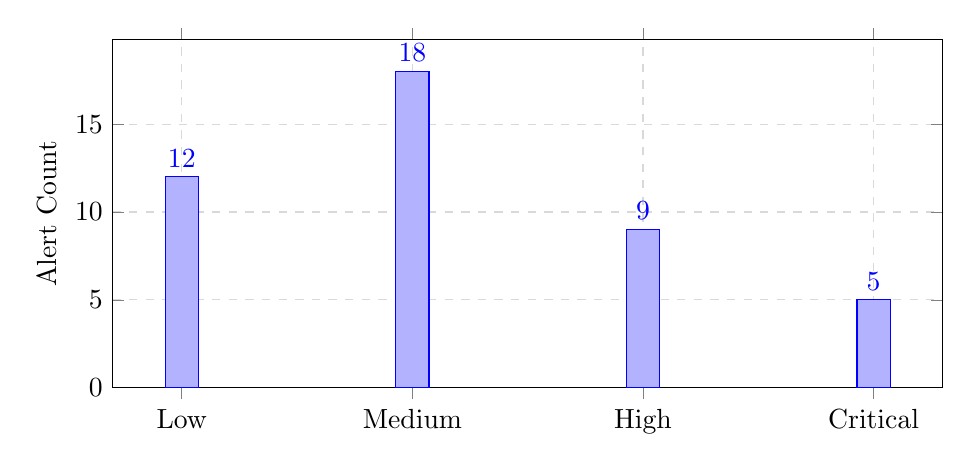
\begin{tikzpicture}
\begin{axis}[
    ybar,
    bar width=12pt,
    width=\columnwidth,
    height=6cm,
    ylabel={Alert Count},
    symbolic x coords={Low,Medium,High,Critical},
    xtick=data,
    nodes near coords,
    ymin=0,
    grid=major,
    grid style={dashed,gray!30}
]
\addplot coordinates {(Low,12) (Medium,18) (High,9) (Critical,5)};
\end{axis}
\end{tikzpicture}
}
\caption{Severity distribution over test window.}
\label{fig:severity}
\end{figure}
\FloatBarrier

\section{Testing and Validation}
ScropIDS includes a documented smoke test flow that validates the SaaS pipeline end-to-end. The test covers organization creation, enrollment token creation, agent enrollment, event ingestion, aggregation, and dashboard metrics retrieval. This provides a lightweight but repeatable quality gate for new deployments.

\section{Deployment}
ScropIDS is deployed with Docker Compose:
\begin{itemize}[leftmargin=1.2em]
    \item \texttt{backend} (Django API),
    \item \texttt{frontend} (Vite build served by Nginx),
    \item \texttt{postgres},
    \item \texttt{redis},
    \item \texttt{celery-worker},
    \item \texttt{celery-beat}.
\end{itemize}
This enables local reproducibility and cloud migration readiness.

\subsection{Service Topology}
\begin{figure}[!t]
\centering
\resizebox{\columnwidth}{!}{%
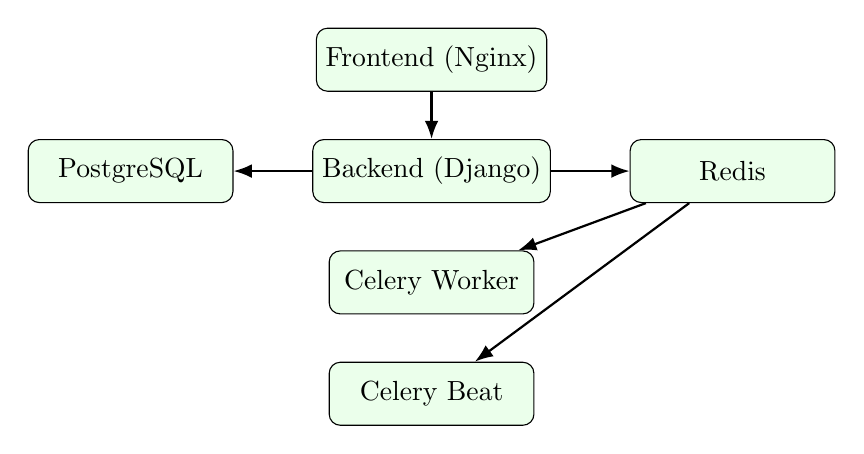
\begin{tikzpicture}[
  node distance=6mm and 10mm,
  box/.style={draw, rounded corners, minimum width=26mm, minimum height=8mm, align=center, fill=green!8},
  arr/.style={-Latex, thick}
]
\node[box] (nginx) {Frontend (Nginx)};
\node[box, below=of nginx] (backend) {Backend (Django)};
\node[box, left=of backend] (db) {PostgreSQL};
\node[box, right=of backend] (redis) {Redis};
\node[box, below=of backend] (worker) {Celery Worker};
\node[box, below=of worker] (beat) {Celery Beat};

\draw[arr] (nginx) -- (backend);
\draw[arr] (backend) -- (db);
\draw[arr] (backend) -- (redis);
\draw[arr] (redis) -- (worker);
\draw[arr] (redis) -- (beat);
\end{tikzpicture}}
\caption{Container topology in Docker Compose.}
\label{fig:compose}
\end{figure}
\FloatBarrier

\subsection{Operational Configuration}
Environment variables provide runtime configuration, including database credentials and optional alert channels (email and webhook integrations). API keys for LLM providers are stored encrypted in the database and never exposed to the frontend.

\section{Performance and Scalability Considerations}
The architecture is designed to scale horizontally. Event ingestion can be scaled by adding backend replicas behind a proxy, while aggregation and LLM analysis can be scaled by increasing Celery worker concurrency. PostgreSQL JSONB indexes and time-windowed aggregation reduce query load for dashboard views. These design decisions support growth from local demos to multi-tenant deployments.

\section{Reproducibility and Availability}
The platform is designed for reproducible builds via Docker Compose, with clear separation of services and environment configuration through variables. This structure supports local demonstrations, CI testing, and future container orchestration.

\section{Ethical and Privacy Considerations}
ScropIDS processes sensitive endpoint telemetry. Deployments must follow data minimization, access control, and audit practices. LLM-based analysis should be treated as advisory and reviewed by analysts before any response action is taken.

\section{Results and Discussion}
The ScropIDS design balances operational simplicity with extensibility. The scheduler and aggregation pipeline provide consistent windows for analysis, while the rule escalation layer reduces dependence on LLM outputs alone. In practice, this hybrid model helps prevent noisy outputs and makes the system usable even when LLM providers are unavailable. The multi-tenant architecture enables efficient SaaS deployment but requires strict access control and careful audit logging. These tradeoffs are acceptable for a production-oriented IDS platform intended for SOC-like workflows and academic evaluation.

\section{Limitations and Future Work}
\begin{itemize}[leftmargin=1.2em]
    \item Model outputs may vary by provider/version.
    \item Long-term profiling and adaptive baselining can be improved.
    \item Future roadmap: Sigma rule packs, MITRE ATT\&CK mapping, threat-intel enrichment, guided mitigation playbooks.
\end{itemize}

\section{Conclusions}
ScropIDS demonstrates that a multi-tenant, cloud-native IDS can combine structured telemetry, scheduler-driven aggregation, and LLM-assisted triage to significantly improve analyst workflow. The platform bridges practical deployment constraints with modern detection usability, making it suitable for both academic evaluation and production-oriented security operations.

\FloatBarrier
\newpage

\appendix
\section{API Examples}
\begin{lstlisting}[language=json,caption={Organization creation request}]
{
  "name": "Acme SOC"
}
\end{lstlisting}

\begin{lstlisting}[language=json,caption={Enrollment request}]
{
  "organization_slug": "acme-soc",
  "enrollment_token": "raw-one-time-token",
  "hostname": "win-lab-01",
  "operating_system": "windows",
  "ip_address": "203.0.113.10"
}
\end{lstlisting}

\begin{lstlisting}[language=json,caption={Event batch example}]
{
  "events": [
    {
      "timestamp": "2026-02-24T19:12:22Z",
      "event_type": "process_creation",
      "severity": "high",
      "data": {
        "process_name": "powershell.exe",
        "command_line": "powershell -enc aW52b2tl"
      }
    }
  ]
}
\end{lstlisting}

\section{Scheduler Configuration Fields}
\begin{table}[!t]
\centering
\begin{tabular}{ll}
\toprule
\textbf{Field} & \textbf{Description} \\
\midrule
scheduler\_enabled & Enable or disable scheduler per tenant \\
aggregation\_interval & Seconds between aggregation windows \\
llm\_mode & Batch or realtime analysis mode \\
min\_severity & Minimum severity to include in aggregation \\
alert\_threshold & Minimum threat level to create alert \\
agent\_event\_interval & Agent event batch interval \\
agent\_sync\_interval & Agent config refresh interval \\
collectors & Toggles for agent collectors \\
\bottomrule
\end{tabular}
\caption{Scheduler and agent runtime configuration fields.}
\label{tab:scheduler-fields}
\end{table}

\section{LLM Prompt Template}
\begin{lstlisting}[caption={LLM analysis prompt template (simplified)}]
You are a cybersecurity threat analysis engine.
Return ONLY valid JSON matching:
{
  "threat_level": "low|medium|high|critical",
  "confidence": 0-100,
  "reasoning": "short explanation",
  "recommended_action": "action steps"
}
Analyze:
<AGGREGATED_JSON_HERE>
\end{lstlisting}

\section{Agent Setup Summary}
Agents can run in interactive setup mode or be pre-configured with credentials. Runtime configuration is refreshed periodically from the backend, allowing centralized control of collectors and intervals.

\section{Dashboard Overview Payload}
\begin{lstlisting}[language=json,caption={Dashboard overview response}]
{
  "totals": {
    "agents": 8,
    "events_24h": 25701,
    "active_alerts": 12,
    "aggregates_pending_llm": 3
  },
  "threat_distribution": [
    { "threat_level": "medium", "count": 9 },
    { "threat_level": "high", "count": 3 }
  ],
  "confidence_heatmap": [
    { "agent__hostname": "win-lab-01", "avg_confidence": 86.5, "count": 2 }
  ],
  "generated_at": "2026-02-24T20:00:00+00:00"
}
\end{lstlisting}

\renewcommand{\refname}{References}
\begin{thebibliography}{9}
\bibitem{mitre}
MITRE ATT\&CK, \url{https://attack.mitre.org/}

\bibitem{sigma}
SigmaHQ, \url{https://github.com/SigmaHQ/sigma}

\bibitem{nist}
NIST CSF 2.0, \url{https://www.nist.gov/cyberframework}

\bibitem{owasp}
OWASP Top 10, \url{https://owasp.org/www-project-top-ten/}
\end{thebibliography}

\end{document}
